\section{Approach}
\label{sec:approach}
Since there are no reference summaries for training,
we design a weakly supervised approach, 
which first synthesizes the mix-structured training data and 
then train a dual-encoder summarization model on such data.

\subsection{Mix-structured Training Data Creation}
\label{sec:data}
Let $R$ denote the set of all reviews about an entity.
To avoid information loss in textual inputs or structured inputs,
we create a synthetic mix-structured training dataset %$\mathbb{D}$ 
with four steps, 
as shown in \figref{fig:dm}:
(1) \textbf{extract opinion-aspect pairs (OAs) and implicit sentences (ISs)} from 
each review in $R$;
(2) \textbf{sample a review} as a summary $s$ from $R$ and 
take the remaining reviews as candidate reviews $R_s$; 
\cut{
(1) \textbf{sample a review} $r$ as a summary from $R$ and take $R - \{r\}$ as candidate reviews $R_s$; 
(2) \textbf{extract opinion-aspect pairs (OAs) and implicit sentences (ISs)} from $R_s$ and $r$;
}
%suppose that $O'$ is OAs extracted from $R'$ and $I'$ is ISs from $R'$, 
(3) {\bf sample OAs} from $R_s$ which describe aspects that
are either in or not in $s$;
and (4) {\bf sample ISs} from $R_s$ 
by similarity with the ISs in $s$. 
The sampled OAs and ISs simulate the OAs and ISs in the actual multi-review to be 
summarized. We then repeat steps (2)-(4) to create many input-summary training pairs.
%We give more details of these four steps next.

\begin{figure}[th]
	\centering
	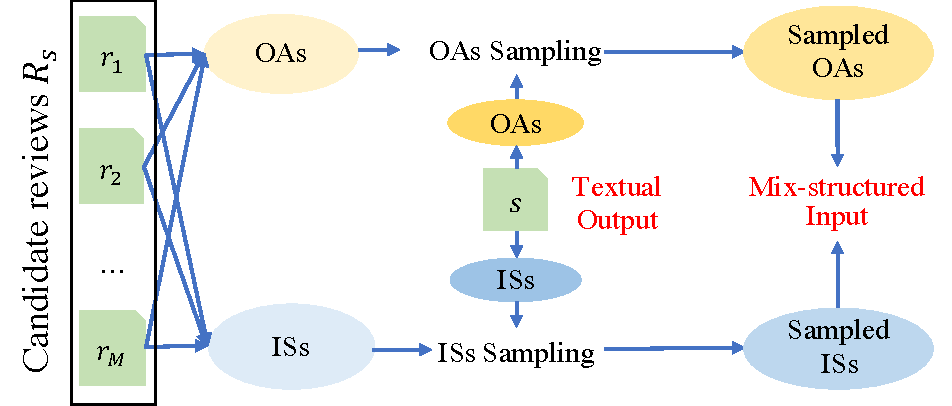
\includegraphics[width=1.0\linewidth]{./dm.pdf}
	\caption{The flow of creating mix-structured data.} %(1)\textasciitilde(4) correspond to the four steps of creating data in first paragraph of \secref{sec:data}. \KZ{Replace with a simpler
%block diagram showing the general work/data flow.}}
	\label{fig:dm}
\end{figure}


\subsubsection{OA and IS Extraction} 
We extract opinion-aspect pairs following the method outlined in \cite{sampo}
\footnote{Our framework is not specific to any opinion-aspect extraction algorithm or tool.
We choose to use \cite{sampo} because it is an unsupervised method, 
which is better at synthesizing datasets for cross-domain review corpora 
(i.e., product, service or movie).}, 
which first utilizes MIN-MINER~\cite{basicOpiMin20} to 
parse sentences into dependency trees and then uses a set of 
syntactic rules~\cite{aspect12} to extract OAs
\footnote{\url{https://github.com/sampoauthors/Sampo}}. 
The opinions thus extracted are typically adjectives which either express the reviewer's
views or sentiments (e.g., ``disappointed'') or describe the aspect (e.g., ``burned'').
Meanwhile, we collect those sentences from which no OAs were extracted, and call these sentences ISs. 
%As shown in \tabref{tab:ours_data}, the mixture output contains the OAs and ISs extracted from 
%its textual output.

\subsubsection{Summary Sampling} 
Given all reviews of an entity, 
we first randomly sample a review. 
Then, we extract aspects (A) from the sampled review and extract aspects (A’) from other reviews. 
If A is the subset of A’, the sampled review can be seen as a summary.
This ensure the sampled review contains only aspects that can be found in other reviews.
Because a summary should not discuss things outside of its input.
Besides, we ignore those reviews containing first-person singular pronouns
and non-alphanumeric symbols except for punctuations~\cite{Denoise20},
since such reviews don't look like real summaries.
%We utilize the OAs and ISs extracted from sampled summary $s$
%and candidate reviews $R_s$ to create the synthetic training data.

\cut{%%%
Given a review $r$, the OAs extracted from $r$ have different aspects.
For an aspect $a$,
%let $O_a$ as the set of OAs based on $a$. 
we take $o$ as an OA pair in $O_a$
and $f$ as the number of occurrences of $o$.
We extract OAs and ISs from sampled summary $s$
and candidate reviews $R_s$.
%The extracted OAs in $R_s$ is indicated as $O'$.
For an aspect $a$ in summary,
the set of OAs with the same aspect in $R_s$ is represented as $O'_a$.%$=\{(o'_{1}, f'_1), ..., (o'_{N}, f'_{n'})\}$. 
The definition of $o'$ and $f'$%, and $n'$
are similar to $o$ and $f$, except that they refer to the ones in $O'_a$.
%The set of ISs in $R_s$ is represented as $I'$.
}

%\YZ{change semi-structure to mixture}
\subsubsection{Opinion-Aspect Pairs Sampling}
\label{sec:OAsample}
%In actual multi-review and summary pairs, 
%the aspects mentioned in a summary 
%should be a subset of aspects in multi-review.
To simulate the actual multi-review, which includes not only all the aspects in the summary,
but also some aspects not in the summary,
we include two types of OAs in the mix-structured data:
{\em popular} pairs and {\em unpopular} pairs.
The OAs whose aspects are included in the summary are popular,
and the other OAs are unpopular.
For example, suppose that (\textit{disappointed}, \textit{food}) is an OA in the summary,
(\textit{bad}, \textit{food}) is a popular pair and (\textit{not fresh}, \textit{beef}) is an 
unpopular pair.

For a given ($o$, $a$) pair in the summary, we sample a popular pair ($o'$, $a$) from $R_s$ 
with a probability which is proportional to the semantic similarity between $o$ and $o'$.
The similarity is computed by the cosine similarity between the average word 
vectors~\cite{glove} from $o$ and $o'$. 
This is to allow opinions which are different from the mainstream ones to be included in
the training data with a small probability. 
Further, we randomly sample an unpopular pair whose aspect doesn't appear 
in the summary at all. Such a pair represents an aspect in the input which is ignored
by the summary.
The number of popular and unpopular pairs to be sampled for each summary is not fixed
but follows a normal distribution, to simulate the variations of the number of OAs 
that are included in different summarization inputs. The determination of parameters of
these normal distributions is important and is discussed in \secref{sec:gauss}.

%which simulates the OAs in normal multiple reviews.
%To compute similarity,
%we take each OA as a sequence of tokens in its opinion and aspect.
%We use GloVe~\cite{glove}
%\footnote{https://nlp.stanford.edu/projects/glove/}
%to represent tokens
%and take the average of embeddings of the tokens in each pair
%to represent each OA.
%as {\em OA embedding}.
%Suppose $a$ is an aspect of OAs in the sampled summary, 
%$O'_a$ is composed of all matched pairs based on aspect $a$ in $O'$.
%$\boldsymbol{o}$ is the vector expressing all OAs on $a$ in summary, 
%which is the average of the corresponding OA embeddings.
%We compute the cosine similarity scores between $\boldsymbol{o}$ and the embeddings of its all matched OA pair in $R_s$.
% as: $cs(a)=cosine\_sim(\boldsymbol{o'}, \boldsymbol{o_s})$,
%where $\boldsymbol{o'}$ is the embedding of $o'$.
%$\mathbf{cs}(a)$ consists of the cosine similarity scores 
%of all matched pairs on $a$.
%We normalize the cosine similarity scores of $a$
%by $\mathbf{cs}'(a)=softmax(\mathbf{cs}(a))$. 
%The $\mathbf{cs}'(a)$ denotes the probability distribution 
%of all matched pairs on aspect $a$.
%Then, we sample $N$ matched pairs on each aspect $a$ according to the distribution %$\mathbf{cs'}(a)$. 
%of such similarity scores.

%To obtain noisy mismatched OAs, 
%we randomly sample some mismatched pairs from $R_s$,
%satisfying the randomness
%of OAs that appear in an actual multi-review 
%but not in its summary.
%The number of sampled mismatched pairs follows the gaussian distribution of the number of pseudo mismatched pairs in $N_r$ reviews from different entities.
%
%Noisy matched and noisy mismatched pairs compose noisy OAs.

\subsubsection{Implicit Sentences Sampling}
\label{sec:ISsample}
For a summary $s$, 
we sample ISs from $R_s$ with a probability proportional to
its similarity with the ISs in $s$. The similarity is computed by  
ROUGE-1 recall score. The total number of such IS sampled is also
determined by a normal distribution determined below.
%We get the probabilities of sentences in $R_s$
%by the $softmax$ function on their R-1 recall scores. 
%We sample $N_I$ sentences from $R_s$ according to the probability distribution.
%$N_I$ is sampled according to the gaussian distribution of the number of implicit sentences in $N_r$ reviews from different entities.
%For each step, we remove the sampled sentence and recalculate the probability distribution of remained sentences in $I'$.
%We collect all the sampled ISs as noisy ISs.

\subsubsection{Estimating Sample Sizes}
\label{sec:gauss}
%In this paper, 
We assume the numbers of popular/unpopular OA pairs and ISs that need to be 
sampled all follow normal distribution, but with different parameters $\mu$ and $\sigma$. 
We assume that our summarization model is supposed to produce a summary for $N$ reviews,
where $N$ is a parameter of the problem. After removing all the eligible output summaries
(each denoted as $s$) from $R$, we call the remaining reviews candidate pool $R_C$. 
We random sample $N$~\footnote{$N$ depends on the number of input reviews of inference sets.}
reviews at a time from $R_C$, and regard those ($o$, $a$) 
pairs in which $a$ appears in more than one review in $R_C$ as popular pairs,
and all other pairs as unpopular pairs. 
Note that we are only approximating the popular
and unpopular pairs here since we do not know the summary $s$ at this time.
We also count the number of ISs in $R_C$. 
After repeating the above random sampling a number of times, we can estimate the $\mu$ and
$\sigma$ for the numbers of popular pairs, unpopular pairs and implicit sentences.

\subsection{Summarization Models}
\label{sec:model}

%\begin{figure*}[t]
%	\centering
%	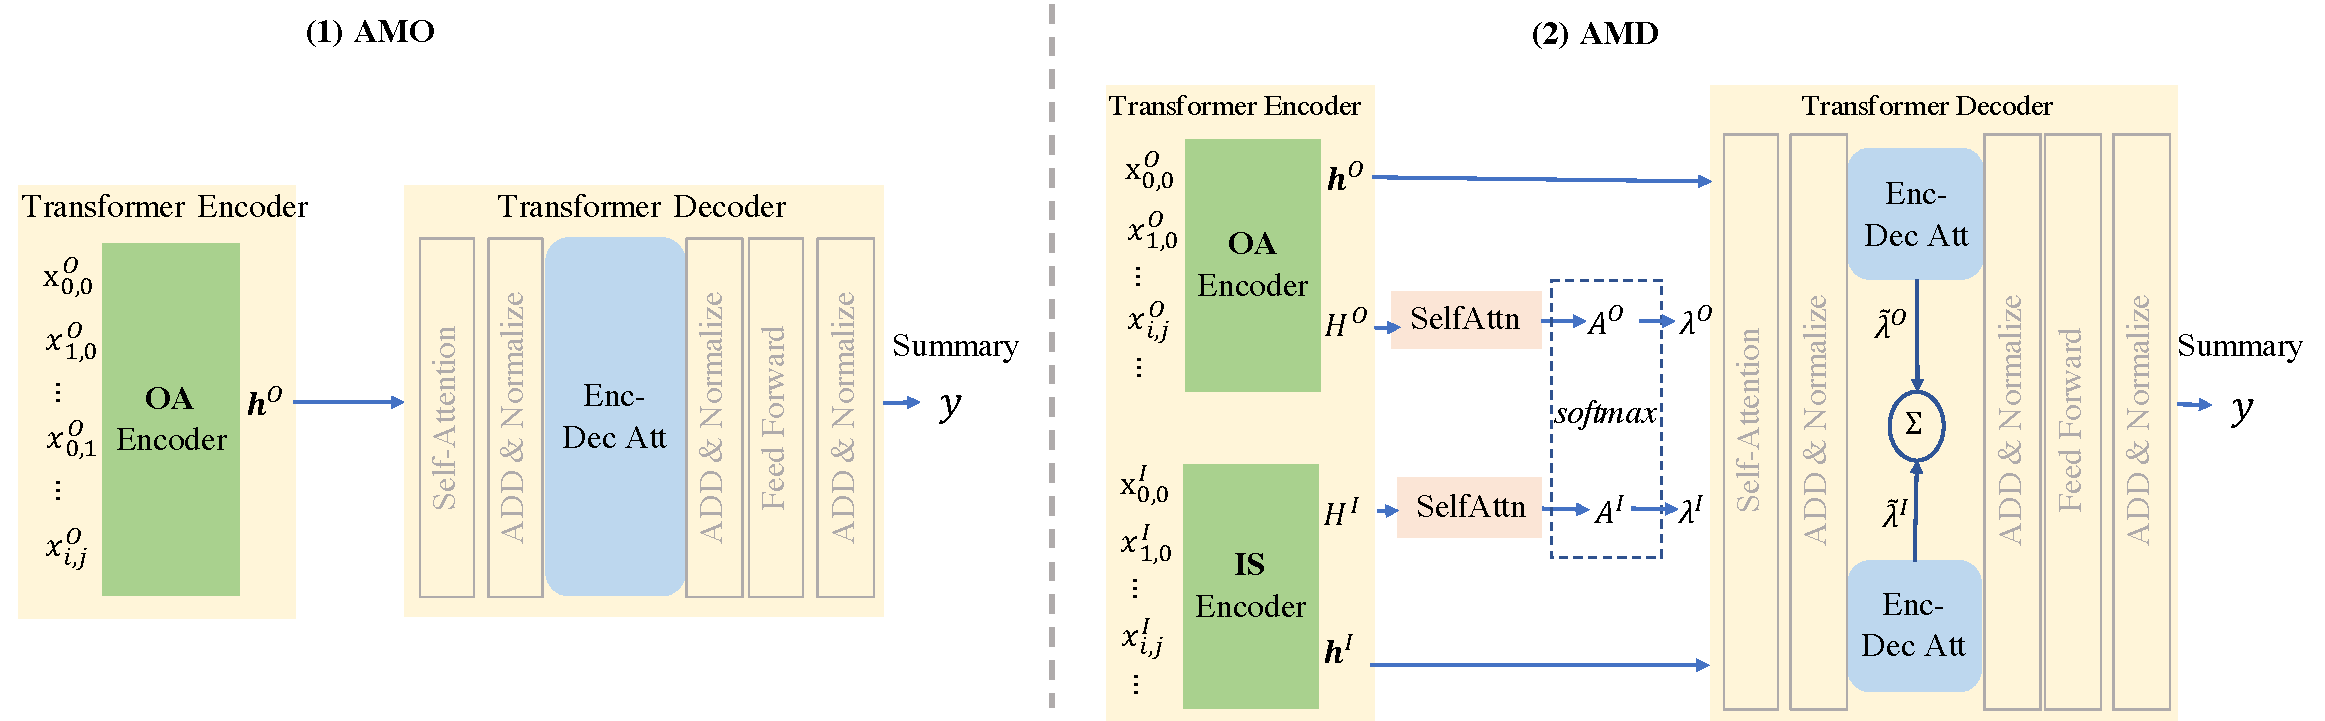
\includegraphics[width=1\linewidth]{./model.pdf}
%	\caption{The architecture of AMO and AMD. \KZ{I suggest you break this figure up into two separate narrow figs 
%to save some space. Note the (1) and (1) above the figs.}}
%	\label{fig:model}
%\end{figure*}

Given OAs and ISs as mixed input, we design a straight-forward seq2seq model 
with a dual encoder that deals with the two types of input separately.
Next, we present the basic model which is based on the transformer, 
and then show a way to optimize the model by using an additional
pretrain stage.
% 
%since they play different roles in summary generation.
%The explicit opinion of a summary is mainly generated by selecting the key pairs from noisy OAs and 
%rephrasing the selected OAs into complete sentences.
%Noisy ISs will be used to summarize implicit opinions.
%When generating summaries, 
%the explicit and implicit opinions also interact with each other.

\cut{\YZ{appendix}
In this subsection, we first present a \textbf{basic aspect-guided model with an encoder} taking only noisy OAs as input, which learns to select accurate aspects and their appropriate opinions 
to generate explicit information.
Then we further propose an {\bf advanced aspect-guided model with a dual encoder} taking both OAs and ISs as input.
In opinion summarization, 
since OAs are the most important information while ISs are supplementary, 
our best approach is to \textbf{train the advanced aspect-guided model initialized with pretrained basic aspect-guided model}.
}

%In order to get high-quality summaries,

%\subsubsection{Basic Aspect-guided Model (BM)}
%We adopt a transformer seq2seq model~\cite{Transformer17} as the basic model,
%which has an OA encoder taking only noisy OAs as input.
%The basic model is in \figref{fig:amo}. 
%
%\begin{figure}[th]
%	\centering
%	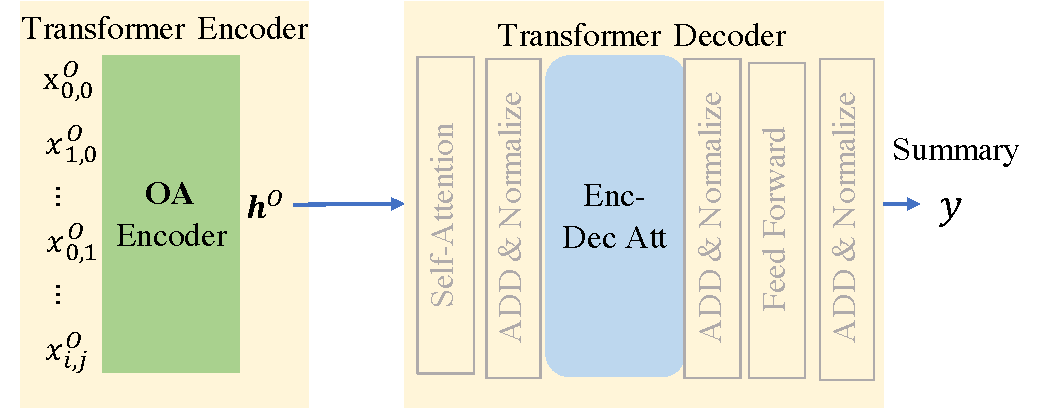
\includegraphics[width=0.9\linewidth]{./AMO.pdf}
%	\caption{Basic aspect-guided model. $\textbf{h}^O$ is the output of encoder. {\em Enc-Dec Attn} is the attention between encoder and decoder.}
%	\label{fig:amo}
%\end{figure}
%
%
%\cut{
%$c_t$ is the context vector, which is the weighted sum of $\textbf{h}^O$ with Encoder-Decoder Attention (\textbf{{\em Enc-Dec Attn}}) as weight.
%After a feed-forward network of transformer~\cite{Transformer17},
%$c_t$ becomes $c'_t$.
%The probability distribution of 
%generating $y_t$ is calculated by:
%\begin{equation}
%p(y_t|y_0,...,y_{t-1}, \textbf{x}^O)=softmax(W^O c'_{t-1}+b^O),
%\label{eq:decode}
%\end{equation}
%where $\textbf{x}^O$ is noisy OAs. $W^O$ and $b^O$ are trainable parameters.
%}%
%
%The basic model with only noisy OAs as input attends to the important pairs in noisy OAs, 
%and consequently tends to generate general and simple summaries.
%We thus add implicit opinion by introducing noisy ISs to the model.
	
\subsubsection{Basic Model}
\label{sec:basicmodel}
Our basic model (\figref{fig:amd}) deals with OAs and ISs
in parallel via two transformer encoders, \textbf{\em OA encoder} and \textbf{\em IS encoder}. 
The parameters of the dual encoder are not shared.
%The architecture is illustrated in \figref{fig:amd}.

\begin{figure}[th]
	\centering
	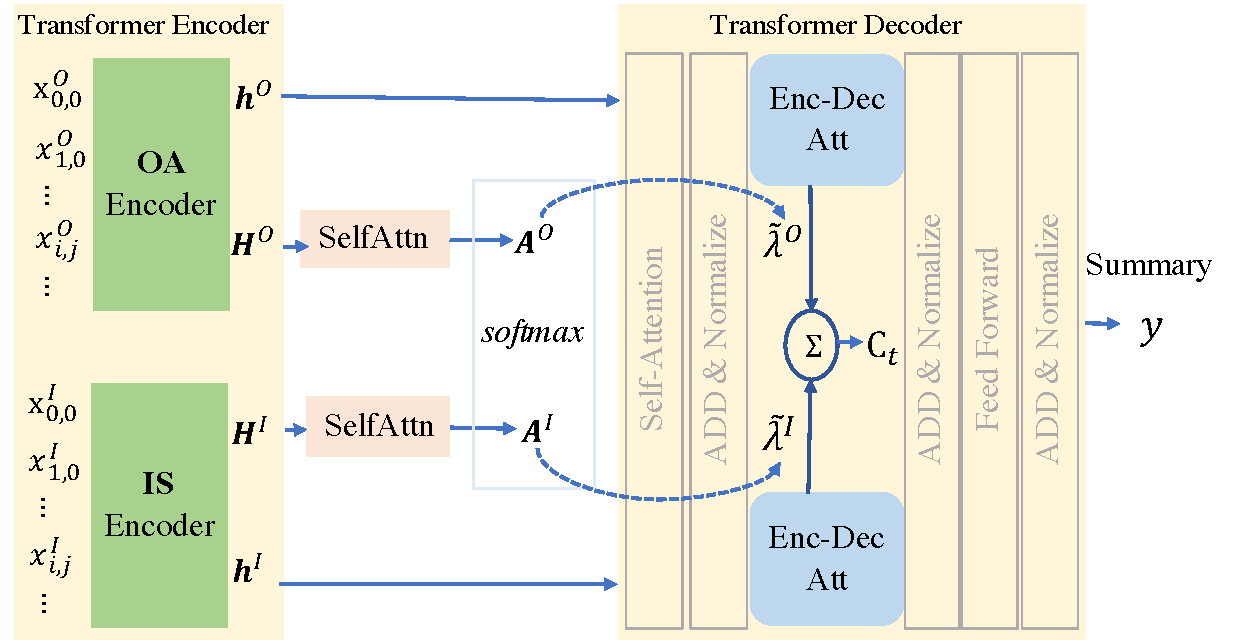
\includegraphics[width=1\linewidth]{./AMD.pdf}
	\caption{Basic model.}
	\label{fig:amd}
\end{figure}

In this model, 
we concatenate the opinion and aspect in each OA,
and arrange all the OAs in a shuffled order.
To model the relation among OAs,
we add a special token at the beginning of each OA, 
which indicates the OA representation.
%As there is no order among OAs, 
%we concatenate the OAs in noisy OAs in a shuffled order. 
$x^O_{i,j}$ is the $i^{th}$ token of $j^{th}$ pair in sampled OAs. 
The special token of $j^{th}$ pair is $x^O_{0,j}$.
The sentences in sampled ISs are concatenated in the
same way as sampled OAs.
$x^I_{0,j}$ is the special token of $j^{th}$ sentence.
We take OAs and ISs as input and summary $\textbf{y}$ as output.

Inspired by~\citet{DialogMV2020},
%we represent the $j$-th OA pair in the noisy OAs by 
%the latent representation of the $j$-th special token $x^O_{0,j}$.
we use $H^O_{j}$ to denote the encoder state of $x^O_{0,j}$,
which indicates the $j^{th}$ pair in sampled OAs.
$\textbf{H}^O=\{H^O_{1},...,H^O_n\}$ consists of all special tokens of OAs.
Then, we aggregate the information of all sampled OAs through self-attention mechanism (\textit{SelfAttn})~\cite{Transformer17} and get the OA representation as $\textbf{A}^O$.
Similarly, we can get the IS representation $\textbf{A}^I$.
\cut{
	\YZ{appendix}
\begin{align}
	\alpha_{i,j} &= \frac{\exp(H^O_i H^O_j)}{\sum_{k=1}^{n}\exp(H^O_i H^O_k)}\\
    A^O_{i} &= \sum\nolimits_{j=1}^{n}\alpha_{i,j}  H^O_j \\
    \alpha_{i,j}' &= \frac{\exp(A_i^O)}{\sum_{i=1}^{n}\exp(A_i^O)} \\
    \textbf{A}^O&= \sum\nolimits_{i=1}^{n} \alpha_{i,j}' A^O_i
\end{align}
where $\textbf{A}^O$ denotes the total information of noisy OAs.
Similarly, we can get all special tokens of noisy ISs, $\textbf{H}^I$, and the IS representation $\textbf{A}^I$.
}%%%
The {\em OA probability} $	\widetilde{\lambda}^O$  is computed as:
\begin{align}
	\lambda &= \frac{\exp(\textbf{A}^O {^\top} v^O)}{\exp(\textbf{A}^O {^\top} v^O)+\exp(\textbf{A}^I {^\top} v^I)} 
	%\widetilde{\lambda}^O &=\frac{ \lambda^{\frac{1}{T}}}{\lambda^{\frac{1}{T}}+(1-\lambda)^{\frac{1}{T}}}
	%\label{eq:T}  \\
%	\widetilde{\lambda}^I &=1-\widetilde{\lambda}^O
\end{align}
where $v^O$ and $v^I$ respectively denote the randomly initialized context vector of OA encoder and IS encoder.
%$W$ and $b$ are parameters. 
We achieve $\widetilde{\lambda}^O$ by applying temperature on $\lambda $ for sharpening the attention distribution between encoders,
and get {\em IS probability} $\widetilde{\lambda}^I$ by $1-\widetilde{\lambda}^O$.


At each decoding step $t$, 
$C_t^O$ is the weighted sum of encoder states of OA with {\em Enc-Dec Attn} as weight. 
$C_t^I$ is the weighted sum of IS encoder.
The combinational context vector $C_t$ for decoding is:
%of the Encoder-Decoder Attention 
%is the weighted sum of $C_t^p$ and $C_t^s$ as:
%is computed as:
%The combinational context vector $C_t$ for decoding is:
\begin{equation}
	C_t = \widetilde{\lambda}^O C_t^O +  \widetilde{\lambda}^I C_t^I
\end{equation}
%\KZ{How? $C_t$ should be modified by feed-forward network and becomes $G_t$.} 
After inputting $C_t$ to the feed-forward network layer of transformer.
The probability distribution of generating $y_t$ is computed by the softmax on $C_t$.
%The probability distribution of generating $y_t$ is:
%\begin{equation}
%p(y_t|y_0,...,y_{t-1}, %\textbf{x}^O,\textbf{x}^I)=softmax(WC_{t-1}+b)
%\end{equation}
%where $\textbf{x}^O$ and $\textbf{x}^I$ denote noisy OAs and noisy ISs respectively.
%$W$ and $b$ are the trainable parameters.

\subsubsection{Optimized Model}
\label{sec:optmodel}
\cut{
\begin{figure}[th]
	\centering
	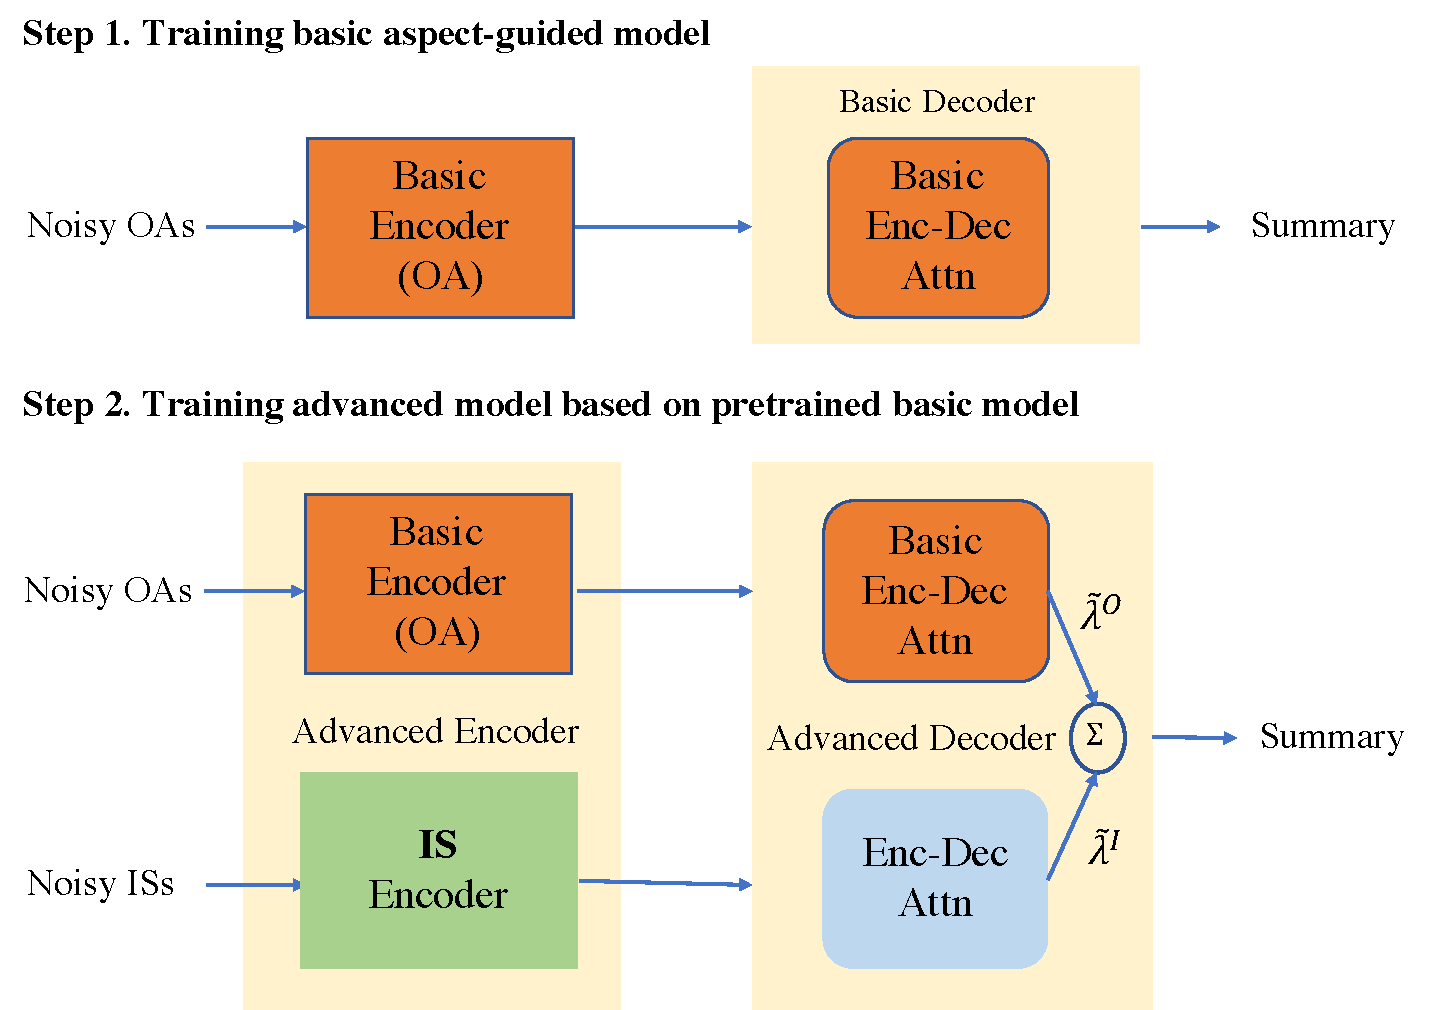
\includegraphics[width=1\linewidth]{./flow.pdf}
	\caption{Training process of optimizing advanced model. The structures in Step 1 and Step 2 are the simplified version of architectures in \figref{fig:amo} and \figref{fig:amd}, respectively.}
	\label{fig:flow}
\end{figure}
%Summaries generated by BAG
Then, we further fine-tune the whole model, enhancing the generated summary with
implicit opinion from noisy ISs. 
At Step 2, the parameters of OA encoder and the attention between OA encoder and decoder 
are initialized by pretrained basic model.
}%%%

In opinion summarization, users' opinions on the aspects of an entity are very important. For optimization, we pretrain a single encoder by setting $\widetilde{\lambda}^I$ as zero and
taking only sampled OAs as input and corresponding summary as output.
%in the training data to the upper part of the basic model. 
%\KZ{Is this do-able on \figref{fig:amd}? What is the intuition behind this two step approach?}
Then, we fine-tune the basic model in \figref{fig:amd} by initializing the OA encoder using the parameters of pretrained encoder, 
enhancing the generated summary with implicit opinion from sampled ISs.



